\documentclass [12pt] {beamer}

\usetheme {Warsaw}
\useoutertheme {miniframes}

\usepackage {graphicx}

\begin {document}
    \title [How to use Matlab for free \hspace {3em} \insertframenumber / \inserttotalframenumber ] {How to use Matlab for free}
    \date {\today}
    \author {TAs}
    \institute {Numerical Analysis - NTU/AS}
    \begin {frame}
        \titlepage
    \end {frame}

    \section {MATLAB}
    \begin {frame}
        \frametitle {MATLAB}
        \begin {block} {How to use Matlab for free ?}
        \begin {itemize}
            \item Matlab need license (i.e. Not free)
            \item NTU provides campus version for NTU members to use
            \item NTU has provided a service (VDI) since 105-1
            \vspace {24pt}
            \item VDI - Virtual Desktop Interface
        \end {itemize}
        \end {block}
        \begin {block} {VDI}
        \begin {itemize}
            \item begin to use : https://vdi.ntu.edu.tw
            \item reference of VDI : http://vdiqa.ntu.edu.tw
            \item software list : http://vdiqa.ntu.edu.tw/sofeware.html
        \end {itemize}
        \end {block}
    \end {frame}

    \section {VDI}
    \begin {frame}
        \frametitle {How to use VDI}
        All software we use in Numerical Analysis are installed in VDI.\\
        And all you need to do in your computer is to open the \alert{browser}.\\
        \vspace {18pt}
        The good news is VDI doesn't have IP address restriction
        \vspace {24pt}
        \begin {block} {software list}
        \begin {itemize}
            \item Word 2013 - can save as PDF
            \item Matlab - run code
            \item 7-zip - wrap files
        \end {itemize}
        \end {block}
    \end {frame}
    \begin {frame}
        \frametitle {How to use VDI}
        Login with NTU mail account
        \begin {figure}
        \begin {center}
            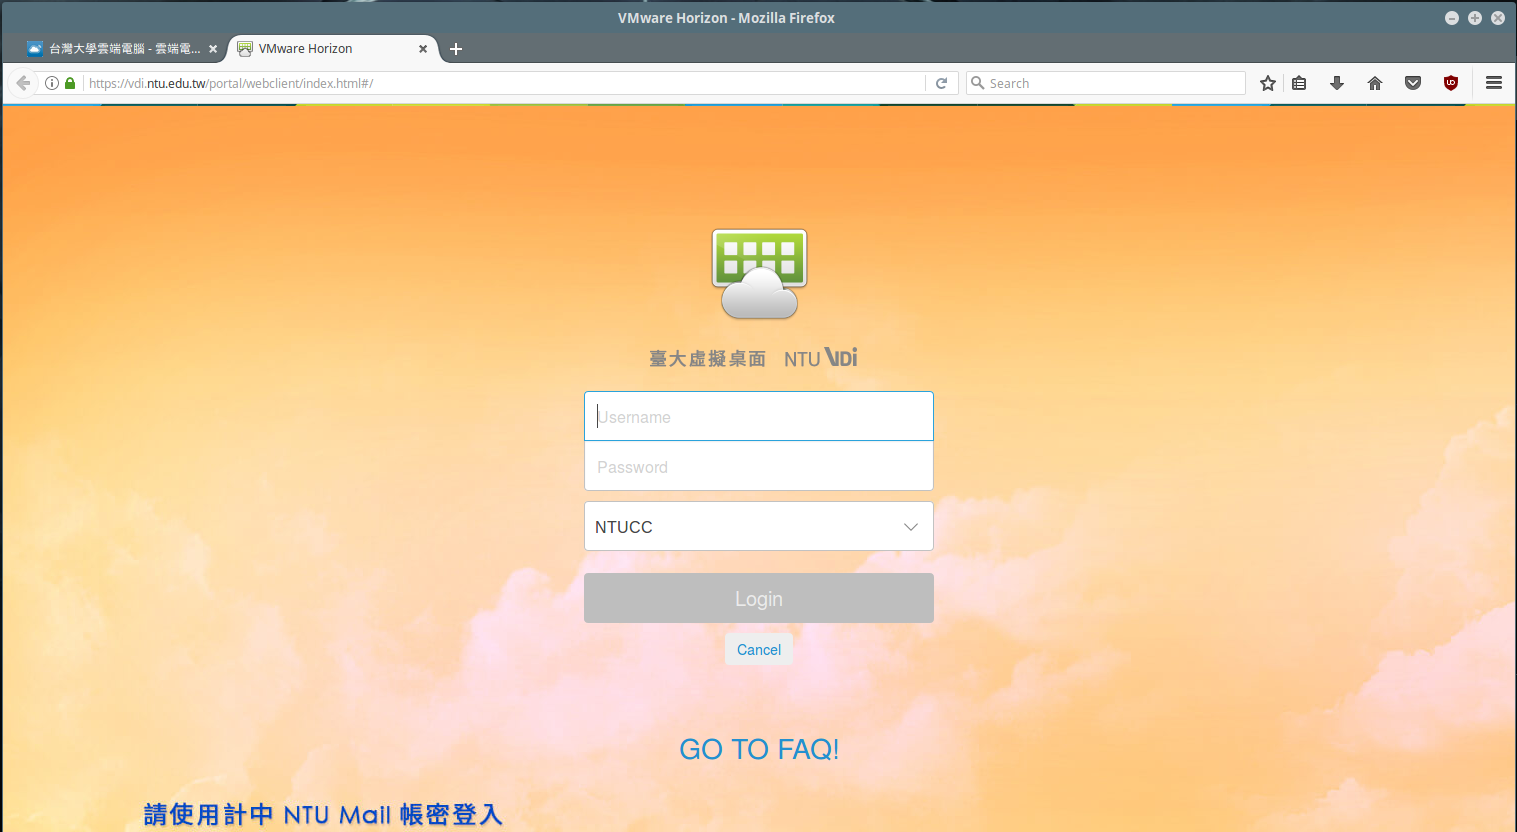
\includegraphics [width=10.5cm] {fig1}
        \end {center}
        \end {figure}
    \end {frame}
    \begin {frame}
        \frametitle {How to use VDI}
        choose win7 chinese version
        \begin {figure}
        \begin {center}
            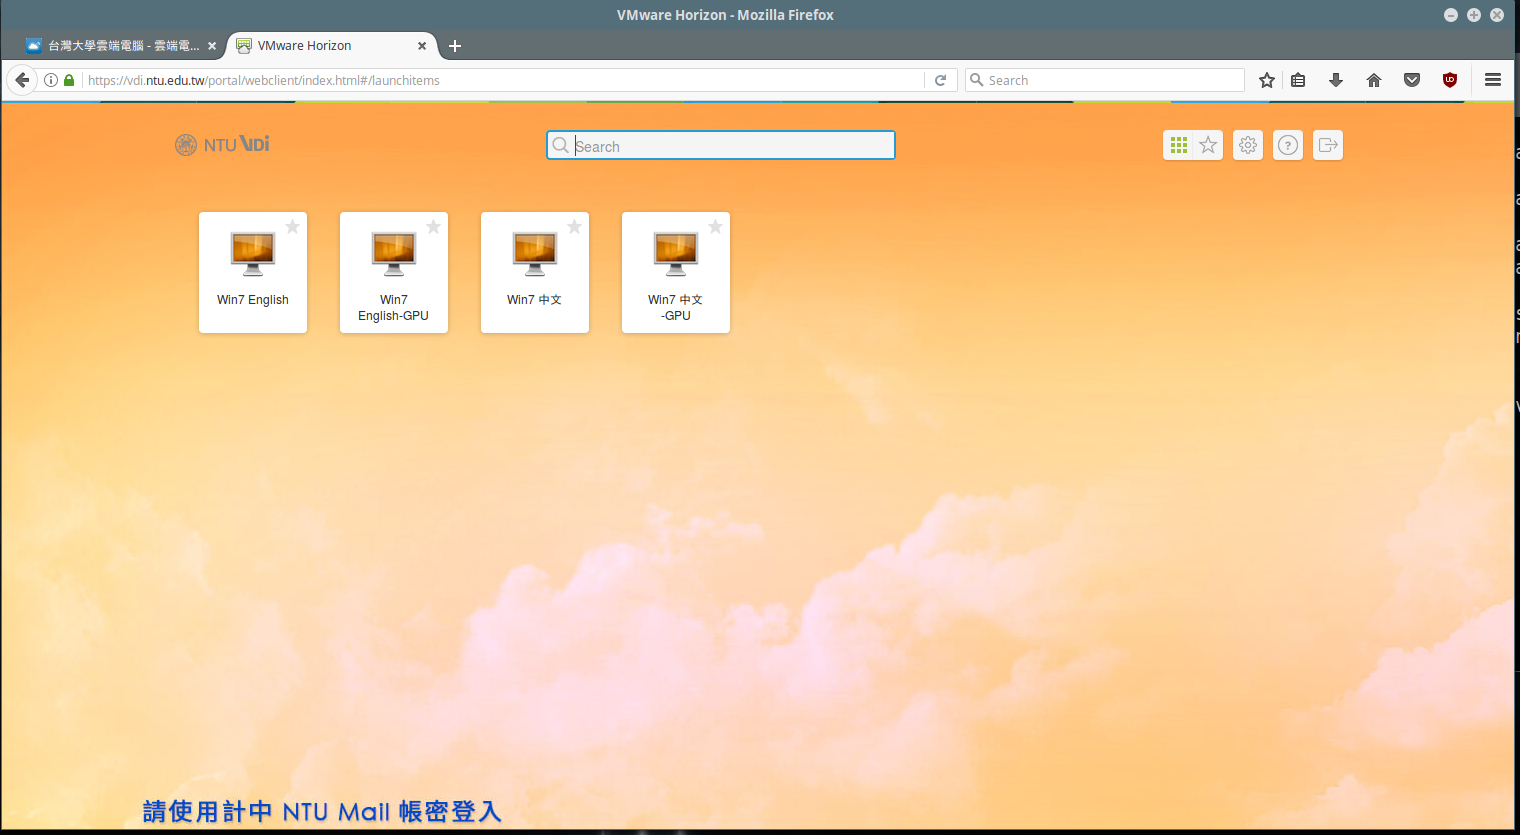
\includegraphics [width=10.5cm] {fig2}
        \end {center}
        \end {figure}
    \end {frame}
    \begin {frame}
        \frametitle {How to use VDI}
        \begin {figure}
        \begin {center}
            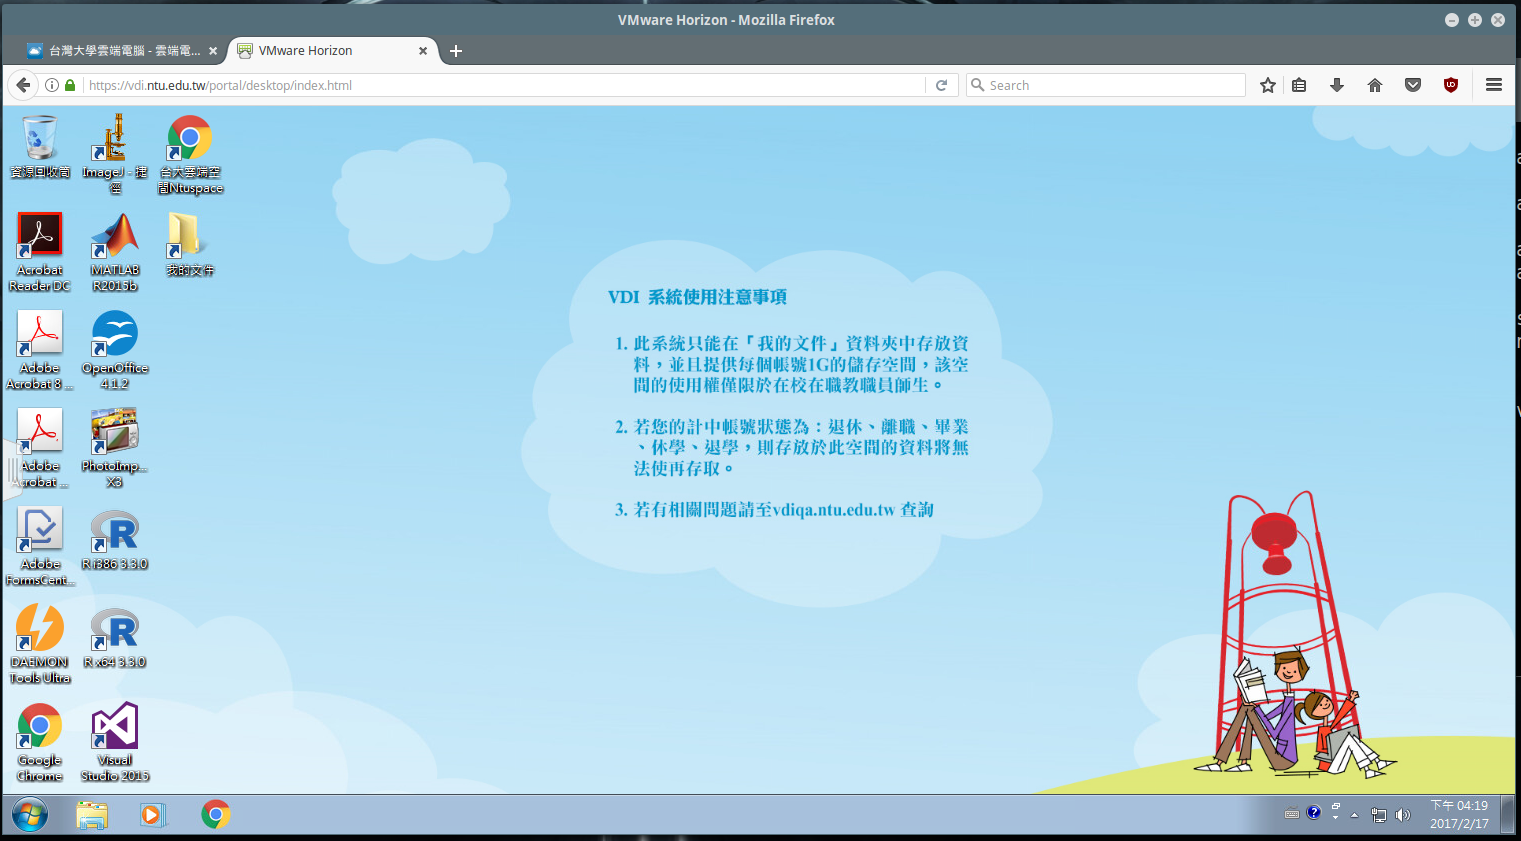
\includegraphics [width=10.5cm] {fig3}
        \end {center}
        \end {figure}
    \end {frame}
    \begin {frame}
        \frametitle {How to use VDI}
        the software we need (Matlab, word) are installed
        \begin {figure}
        \begin {center}
            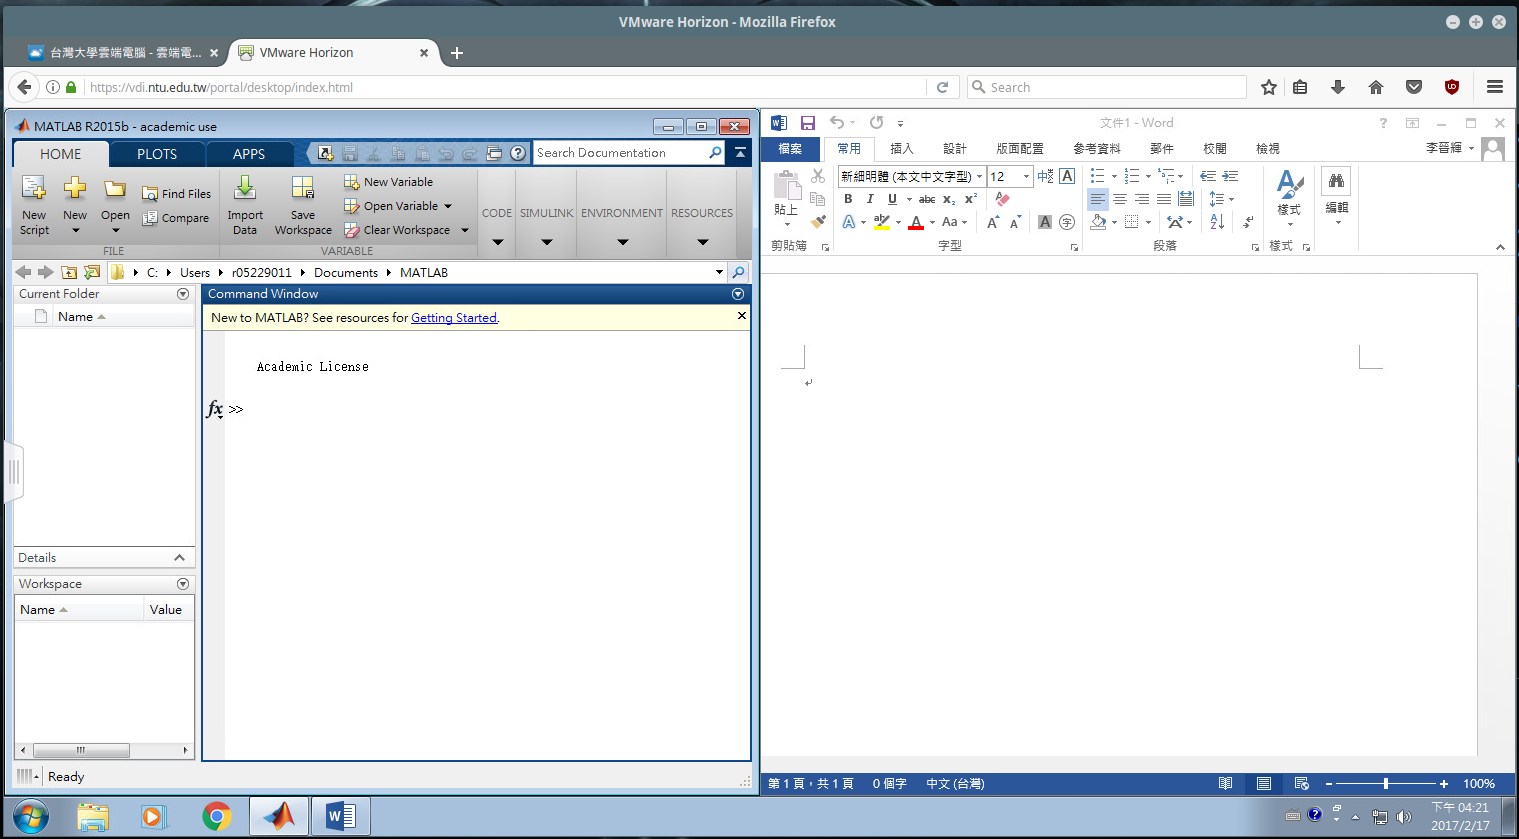
\includegraphics [width=10.5cm] {fig4}
        \end {center}
        \end {figure}
    \end {frame}

    \section {Restriction}
    \begin {frame}
        \frametitle {Restriction}
        \begin {block} {Restriction}
        \begin {itemize}
            \item No usb flash drive provided
            \item All your files need to be saved in "My documents".
            \item To get files, you need use the \alert{Internet} such as NTU space or Google drive.
        \end {itemize}
        \end {block}
        \begin {block} {Or ...}
        \begin {itemize}
            \item Submit your homework in VDI
        \end {itemize}
        \end {block}
    \end {frame}
\end {document}
